\documentclass[12pt, ngerman, utf8]{article}
\usepackage[utf8]{inputenc}
%\usepackage[pass]{geometry}
\usepackage{listings}
\usepackage{color}
\usepackage{graphicx}
\usepackage{url}
\usepackage{float}
\usepackage[german]{babel}


%Customize a bit the look
\lstset{ %
backgroundcolor=\color{white}, % choose the background color; you must add \usepackage{color} or \usepackage{xcolor}
basicstyle= \footnotesize, % the size of the fonts that are used for the code
breakatwhitespace=false, % sets if automatic breaks should only happen at whitespace
breaklines=true, % sets automatic line breaking
captionpos=b, % sets the caption-position to bottom
commentstyle=\color{mygreen}, % comment style
deletekeywords={...}, % if you want to delete keywords from the given language
escapeinside={\%*}{*)}, % if you want to add LaTeX within your code
extendedchars=true, % lets you use non-ASCII characters; for 8-bits encodings only, does not work with UTF-8
frame=single, % adds a frame around the code
keepspaces=true, % keeps spaces in text, useful for keeping indentation of code (possibly needs columns=flexible)
keywordstyle=\color{blue}, % keyword style
% language=Octave, % the language of the code
morekeywords={*,...}, % if you want to add more keywords to the set
numbers=left, % where to put the line-numbers; possible values are (none, left, right)
numbersep=5pt, % how far the line-numbers are from the code
numberstyle=\tiny\color{mygray}, % the style that is used for the line-numbers
rulecolor=\color{black}, % if not set, the frame-color may be changed on line-breaks within not-black text (e.g. comments (green here))
showspaces=false, % show spaces everywhere adding particular underscores; it overrides 'showstringspaces'
showstringspaces=false, % underline spaces within strings only
showtabs=false, % show tabs within strings adding particular underscores
stepnumber=1, % the step between two line-numbers. If it's 1, each line will be numbered
stringstyle=\color{mymauve}, % string literal style
tabsize=2, % sets default tabsize to 2 spaces
title=\lstname % show the filename of files included with \lstinputlisting; also try caption instead of title
}
%END of listing package%
 
\definecolor{darkgray}{rgb}{.4,.4,.4}
\definecolor{purple}{rgb}{0.65, 0.12, 0.82}
 
%define Java language
\lstdefinelanguage{Java}{
keywords={typeof, new, true, false, catch, function, return, null, catch, switch, var, if, in, while, do, else, case, break, int, List, Move, GameConfig, String, Field},
keywordstyle=\color{blue}\bfseries,
ndkeywords={class, export, boolean, throw, implements, import, this},
ndkeywordstyle=\color{darkgray}\bfseries,
identifierstyle=\color{black},
sensitive=false,
comment=[l]{//},
morecomment=[s]{/*}{*/},
commentstyle=\color{purple}\ttfamily,
stringstyle=\color{red}\ttfamily,
morestring=[b]',
morestring=[b]"
}
 
\lstset{
language=Java,
extendedchars=true,
basicstyle=\footnotesize\ttfamily,
showstringspaces=false,
showspaces=false,
numbers=left,
numberstyle=\footnotesize,
numbersep=9pt,
tabsize=2,
breaklines=true,
showtabs=false,
captionpos=b
}

\renewcommand{\contentsname}{Inhalt}
\renewcommand{\lstlistingname}{Beispiel}
\renewcommand{\lstlistlistingname}{Liste der \lstlistingname e}


\begin{document}
\title{Independent Coursework:\\Untersuchung unterschiedlicher Algorithmen zur Anordnung von Bildern mit Beibehaltung der Seitenverhältnisse}
\author{Lilian Hung}

\maketitle

\newpage

\tableofcontents 

\lstlistoflistings

\newpage



\section{Einführung}
Auf der Suche nach einem geeigneten Algorithmus, der Bilder ihrer Ähnlichkeit nach anordnet, dabei das Seitenverhältnis der Bilder (``aspect ratio'') beibehält und den Zwischenraum der Bilder minimiert werden im Folgenden drei verschiedene Paper untersucht, indem die gegebenen Algorithmen implementiert und ausgewertet werden, wie gut sie gewisse Eingaben darstellen. Zwei weitere Paper wurden ebenfalls untersucht und in Abschnitt \ref{sec:weiter-algs} zusammengefasst.
\subsection{Versuchsaufbau}
Als Eingabe wird eine Menge von Rechtecken unterschiedlicher Farbe und Größe verstanden, die als Repräsentation von Bildern gesehen werden. Diese Rechtecke haben eine Sortierung bzw. Position im zwei-dimensionalen Raum, welche zeigt wie ähnlich sich die Rechtecke nach einer bestimmten Eigenschaft sind.\\\\
\begin{figure}[h]
\centering
\begin{minipage}{.40\textwidth}
  \centering
  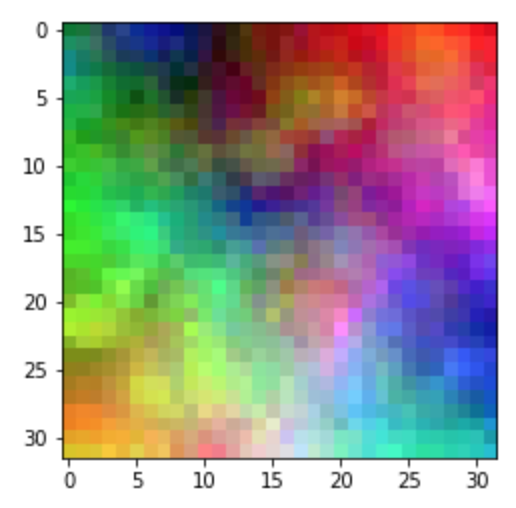
\includegraphics[width=0.9\textwidth]{./imgs/32mal32-som.png}
  \caption{$32\times32$ SOM}
  \label{fig:32som}
\end{minipage}%
\hfill
\begin{minipage}{.55\textwidth}
  \centering
  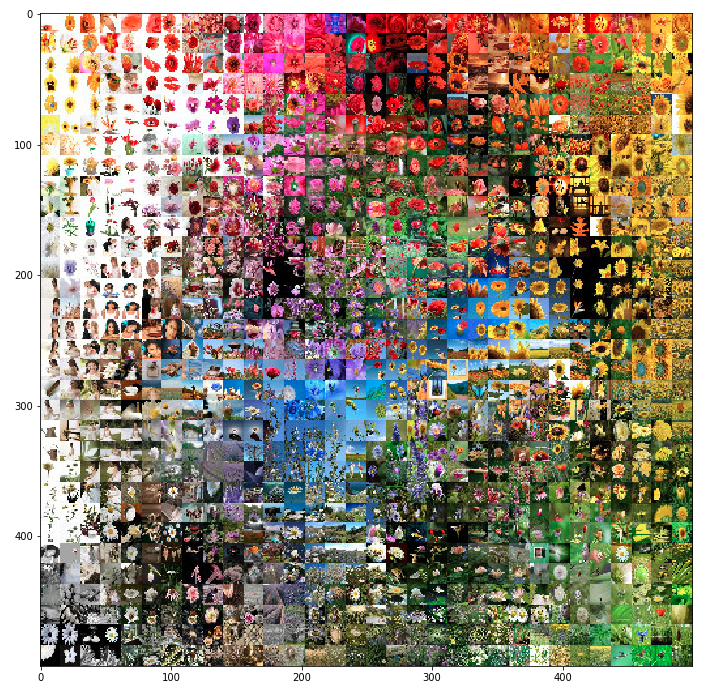
\includegraphics[width=0.9\textwidth]{./imgs/32x32-flowers.png}
  \caption{$32\times32$ vorsortierte Bilder von Blumen}
  \label{fig:32flowers}
\end{minipage}
\end{figure}
In den praktischen Versuchen wurde hauptsächlich auf eine  $32\times32$ Einheiten/Pixel große Self-Organized-Map (SOM) zurückgegriffen (Siehe Abbildung \ref{fig:32som}) und somit war das Ähnlichkeitsmaß in diesem Fall die Farbe der Rechtecke. 
Die SOM wurde zuvor berechnet und aus dem gegebenen Bild wurde dann ein zwei-dimensionaler Array erstellt, der die Farben der Pixel speichert. In der selben Größe ($32\times32$) wurde daraufhin ein Array erstellt, der Rechtecke  unterschiedlicher Seitenlängen und entsprechenden, aus dem SOM-Farb-Array zugeordneten, Farben enthält. Der \emph{RWordle}-Algorithmus in Abschnitt \ref{sec:rwordle} verwendet zusätzlich auch die sortierten Bilder von Blumen (siehe Abbildung \ref{fig:32flowers}).

\subsubsection{Erstellung der Rechtecke}
Die \emph{Python}-Implementierung zur Erstellung der Rechtecke (Beispiel \ref{calc-rects}) wird in der Umsetzung der Algorithmen \emph{RWordle} und \emph{PicWall} verwendet. Die Rechtecke werden als Tupel in einem Array \texttt{rects} mit Informationen über die Position, Höhe und Breite und einer Farbe abgelegt.\\
\begin{lstlisting}[language=Python, caption={Erstellung der Rechtecke; \texttt{col\_arr} enthält die Farben aus der SOM},label=calc-rects]
rects = []
for x in range(0, 32):
    for y in range(0, 32):
        rand_width = randint(30,100)
        rand_height = randint(30,100)
        all_width = all_width + rand_width
        all_height = all_height + rand_height
        r = float(col_arr[x][y][0]/255)
        g = float(col_arr[x][y][1]/255)
        b = float(col_arr[x][y][2]/255)
        rects.append( (x, y, rand_width, rand_height, (r,g,b, 0.6)) ) #alpha 0.6
\end{lstlisting}
Zur Darstellung der Rechtecke wird die \texttt{pyplot}-Funktion in Kombination mit der \texttt{patches}-Funktion, beides Funktionen der \texttt{mathplotlib}-Bibliothek, verwendet.\\\\
Die Implementierung der Generierung der Datenpunkte für \textit{Nmap} wurde in \emph{JavaScript} mit Hilfe des Paketes \texttt{get-pixels} \cite{npm-get-pixels} umgesetzt. 

\section{\textit{Nmap}}
Das Paper \textit{Nmap: A Novel Neighborhood Preservation Space-filling Algorithm}\cite{nmap} behandelt die Erstellung einer Tree-Map unter Beachtung der Position und eines Gewichtes der gegebenen Datenpunkte.
Die Beachtung der Position und damit das Ziel Ähnlichkeitsbeziehungen zwischen den Elementen beizubehalten ist ein entscheidender Punkt, in dem sich \textit{Nmap} von anderen Tree-Maps unterscheidet.
\textit{Nmap} steht für \textit{Neighborhood Treemap}. Der allgemeine Ansatz, der in \textit{Nmap} verwendet wird, ist der \textit{Slice-And-Scale}-Ansatz. 

\begin{figure}[h]
    \noindent
  \makebox[\textwidth]{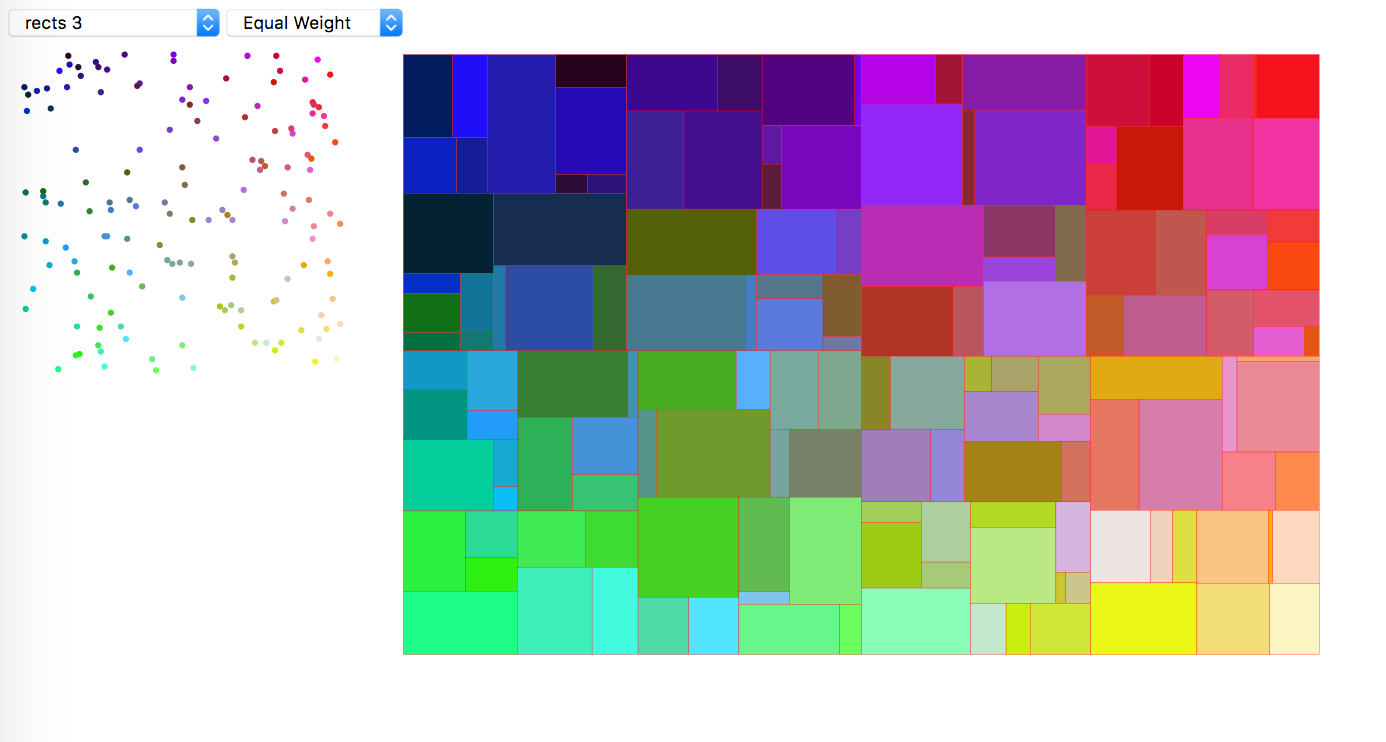
\includegraphics[width=0.9\textwidth]{./imgs/nmap-colored-data-screenshot.png}}
    \caption{Erste Versuche mit \emph{Nmap}. Die Datenpunkte wurden mit randomisierter Position und Größen/Gewichten generiert.}
    \label{fig:nmap-one}
\end{figure}

\subsection{Algorithmus}
Im Paper \cite{nmap} werden zwei Formen von \textit{Nmap} beschrieben -- \textit{Nmap-AC} (``Alternate Cut'') und \textit{Nmap-EW} (``Equal Weight'').
In \textit{Nmap-AC} wird das zu füllende Rechteck abwechselnd horizontal und vertikal geteilt, die erste Teilrichtung ist horizontal, wenn das Rechteck höher als breit ist, und vertikal ansonsten. Bei horizontaler Teilung werden die Datenpunkte an ihrem Median nach Sortierung anhand der $y$-Koordinate geteilt, bei vertikaler Teilung wird der Median nach Sortierung anhand der $x$-Koordinate ermittelt. Dann werden die beiden neuen Rechtecke nach den Gewichtsummen der enthaltenen Datenpunkte skaliert. Dieser Schritt wird rekursiv wiederholt bis ein Rechteck nur noch einen Datenpunkt enthält. In \textit{Nmap-EW} werden die Datenpunkte nicht am Median geteilt, sondern so, dass beide Teilmengen der Datenpunkte das selbe Gewicht enthalten.

\subsection{Implementierung und Auswertung}
Es gibt bereits zugängliche Implementierungen von \textit{Nmap} in \emph{Java} und \emph{JavaScript}. Die Implementierung in \emph{JavaScript} visualisiert die Daten mit \emph{D3} und lässt sich auf \emph{Github} finden und klonen (siehe \cite{nmapcode}). Die geklonte und angepasste Implementierung befindet sich hier \cite{nmapclone}.
Um die Implementierung am gegebenen Anwendungsfall zu testen, müssen Datenmengen in Form von CSV-Dateien generiert werden. Außerdem musste der \emph{D3}-Code zur Visualisierung angepasst werden, damit Datenpunkte \emph{mit Farb-Informationen} entsprechend angezeigt werden können. 
Die Generierung der Daten ist in \emph{JavaScript} implementiert und kann im Terminal mit \emph{node} ausgeführt werden. Für die ersten Tests wurden nur Daten mit unterschiedlichen Farben und Größen bzw. Gewichten generiert, welche nach ihrer rot- und grün-Komponente im zwei-dimensionalen Raum angeordnet wurden. Später wurden mit der gegebenen $32\times32$ SOM, Datenpunkte in der durch die SOM vorgegebenen zwei-dimensionalen Sortierung und mit unterschiedlichen Gewichten generiert. 

\begin{figure}[h]
    \noindent
  \makebox[\textwidth]{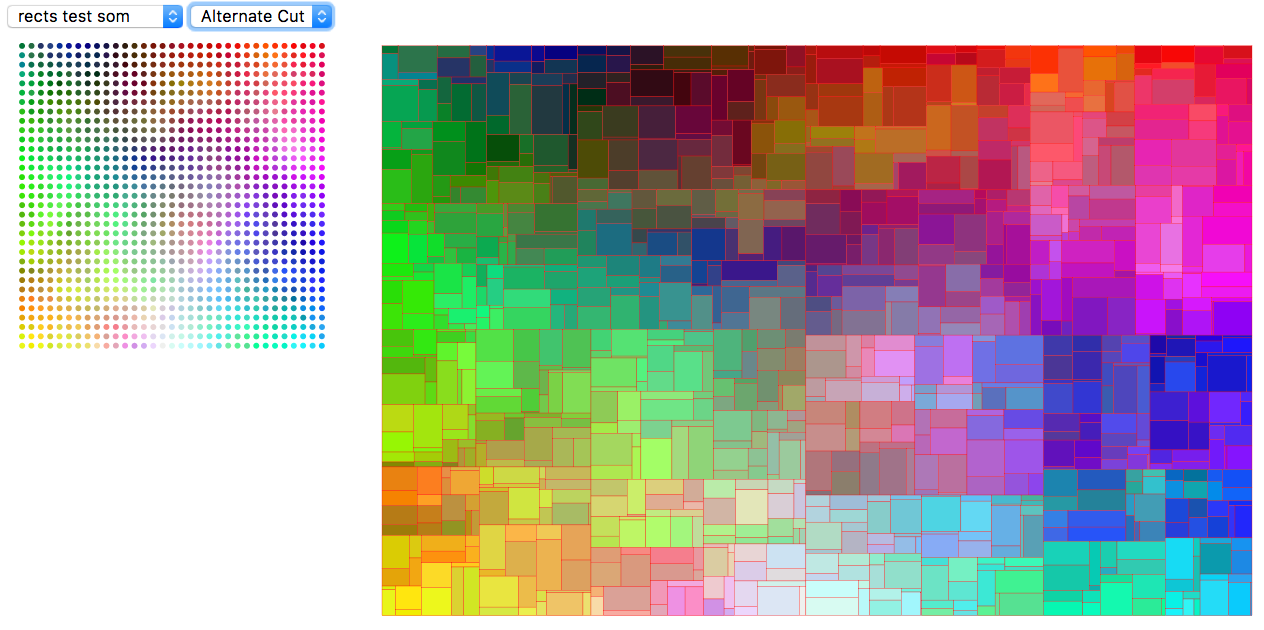
\includegraphics[width=0.9\textwidth]{./imgs/nmap-ac.png}}
    \caption{Visualisierung von \emph{Nmap-AC} mit Datenpunkten, die aus der gegebenen SOM mit randomisierten Größen/Gewichten generiert wurden.}
    \label{fig:nmap-ac}
\end{figure}

\begin{figure}[h]
    \noindent
  \makebox[\textwidth]{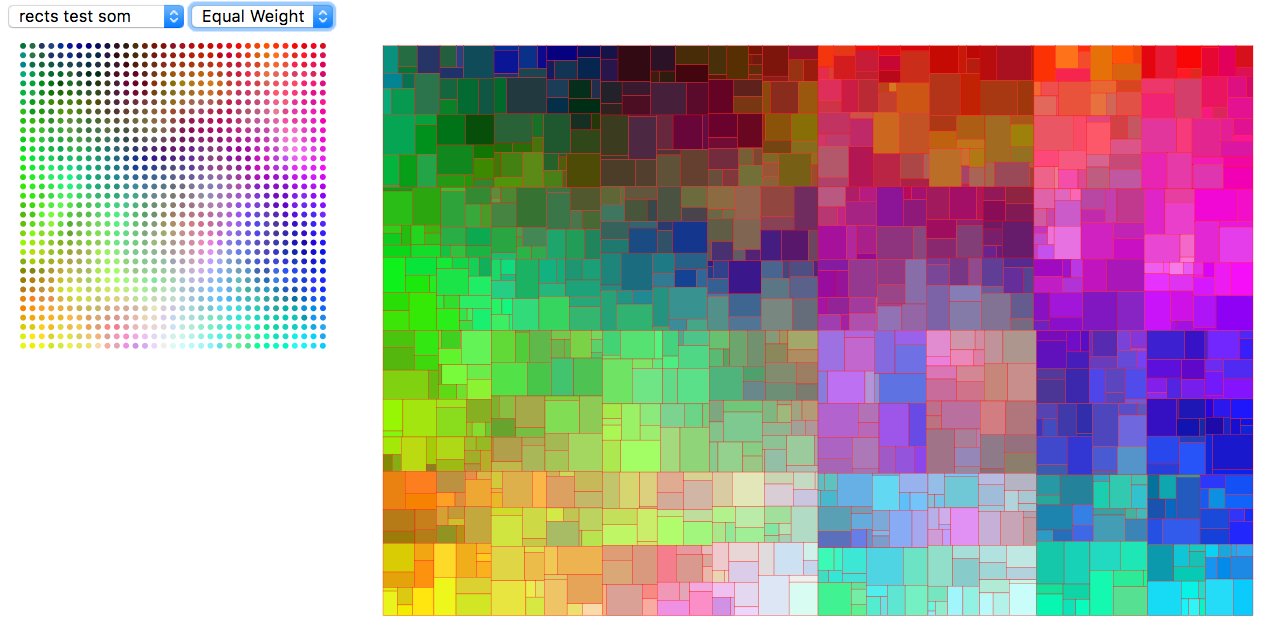
\includegraphics[width=0.9\textwidth]{./imgs/nmap-ew.png}}
    \caption{Visualisierung von \emph{Nmap-EW} mit Datenpunkten, die aus der gegebenen SOM mit randomisierten Größen/Gewichten generiert wurden.}
    \label{fig:nmap-ew}
\end{figure}

\subsubsection{Anmerkung zur Generierung der Datenpunkte}
Bei einer Generierung muss sowohl bei den Gewichten der Datenpunkte, als auch bei deren Position darauf geachtet werden, dass diese alle leicht unterschiedlich sind. Bei den Positionen ist damit der Abstand zwischen den Datenpunkten gemeint. Sollten diese identisch sein, kann es zu Lücken in der späteren Visualisierung durch \emph{Nmap} kommen. In der Dokumentation von nmap.js wird zwar darauf hingewiesen, dass eine Visualisierung von Elementen mit gleichem Gewicht diesen Darstellungsfehler hervorruft, jedoch konnte ich den Fehler auch bei gleichen Abständen zwischen Datenpunkten feststellen. Der Fehler lässt sich beim Gewicht und bei den Koordinaten der Daten durch eine Addition einer kleinen Zufallszahl beheben (\texttt{[...]x: 50 + Math.random(), y: 50 + Math.random(), weight: 1000 + Math.random() [...] }).
\begin{figure}[h]
\centering
\begin{minipage}{.45\textwidth}
  \centering
  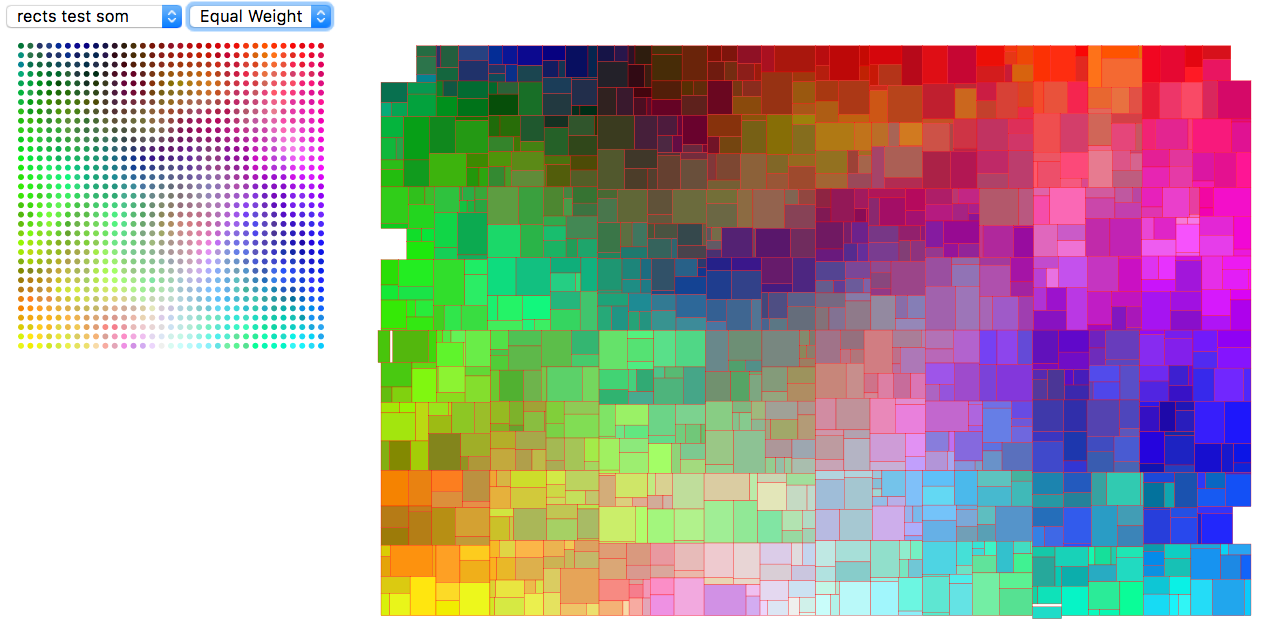
\includegraphics[width=0.9\textwidth]{./imgs/nmap-ew_fehler.png}
  \caption{Fehlerhafte Visualisierung von \emph{Nmap-EW}, da die Datenpunkte keinen leicht randomisierten Abstand zueinander haben.}
  \label{fig:nmap-ew-fehler}
\end{minipage}%
\hfill
\begin{minipage}{.45\textwidth}
  \centering
  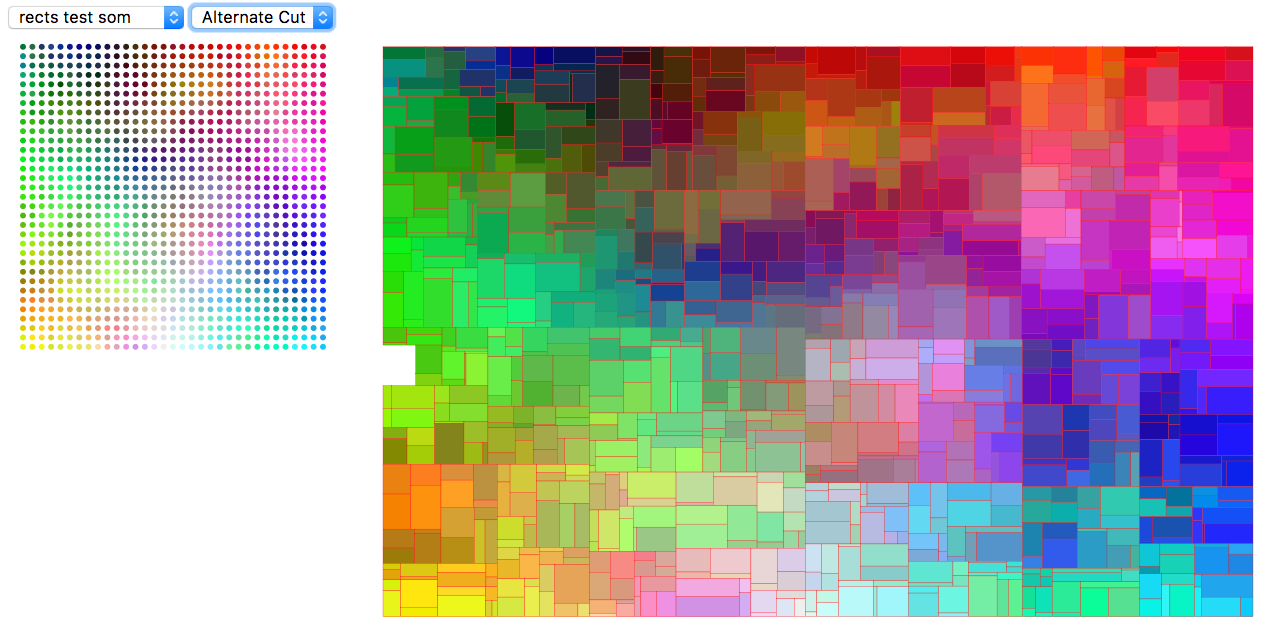
\includegraphics[width=0.9\textwidth]{./imgs/nmap-ac_fehler.png}
  \caption{Fehlerhafte Visualisierung von \emph{Nmap-AC}, da die Datenpunkte keinen leicht randomisierten Abstand zueinander haben.}
  \label{fig:nmap-ac-fehler}
\end{minipage}
\end{figure}

\subsubsection{Auswertung}
Da \emph{Nmap} eine lückenfreie Aufteilung einer vorgegebenen Fläche zurückgibt und dabei die Nachbarschaften der visualisierten Elemente gut aufrecht erhält, scheint es für den Anwendungsfall vorsortierte Bilder bzw. Rechtecke zu visualisieren geeignet zu sein. Damit die Eingabemenge für \emph{Nmap} passend ist, braucht man für jedes Element, in diesem Fall ein Bild oder ein Rechteck, eine Position in Form einer $x$ und $y$-Koordinate und ein Gewicht. Das Gewicht kann als die Höhe mal die Breite eines Rechtecks oder Bildes definiert werden. An dieser Definition kann bereits erkannt werden, dass in der späteren Visualisierung zwar eine Fläche dem Bild entsprechend dargestellt wird, aber das ursprüngliche Seitenverhältnis nicht garantiert erhalten bleibt. Somit fällt ein essenzieller Teil des zu lösenden Problems weg und es muss für \emph{Nmap} gefolgert werden, dass es sich, ohne größere Veränderungen, nicht als Lösung eignet.

\section{\textit{RWordle}}\label{sec:rwordle}
Das Problem, das in \emph{Rolled-out Wordles: A Heuristic Method for Overlap Removal of 2D Data Representatives} \cite{rwordle} versucht wird zu Lösen, ist die Aufhebung von möglichen Überlagerungen von flächigen Objekten (in diesem Fall Rechtecke oder wie im Paper genannt ``Label'') durch neue Positionierung. Der ursprüngliche Anwendungsfall ist die Aufhebung von Überlagerungen, die oftmals beim Mapping von höher-dimensionalen Daten auf eine zwei-dimensionale Fläche entstehen.

\subsection{Algorithmus}
Es gibt zwei Versionen von \emph{RWordle}. In der einen Version wird die Datenmenge genommen und entlang einer linearen Achse (beispielsweise der $y$-Achse) sortiert und die Elemente der Datenmenge dieser Reihenfolge nach neu positioniert (\emph{RWordle-L}). Das erste Element behält seine Position und die folgenden Elemente werden um die bereits positionierten Elemente herum positioniert. Im Genaueren wird die neue Position ausgehend von der ursprünglichen Position des Rechtecks bestimmt. Die Suche erfolgt spiral- bzw. kreisförmig um die ursprüngliche Position herum (siehe Abbildung \ref{fig:rwordle-illus}). Die andere Version sortiert die Datenmenge nach einer konzentrischen Sortierung (\emph{RWordle-C}). Damit ist gemeint, dass die Elemente nach ihrem Abstand zum Mittelpunkt der gesamten Datenmenge sortiert werden. Die Elemente werden ebenfalls entsprechend ihrer Reihenfolge neu positioniert. 

\begin{figure}[h]
    \noindent
  \makebox[\textwidth]{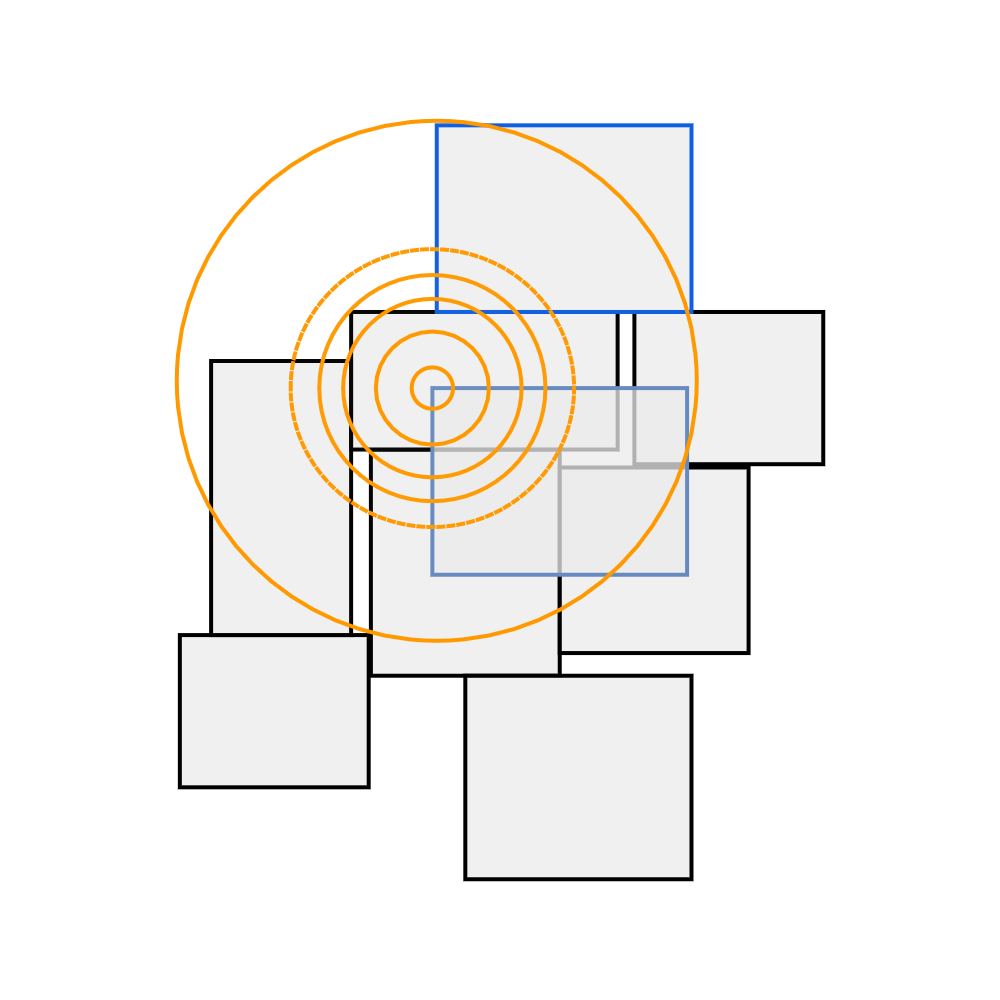
\includegraphics[width=0.7\textwidth]{./imgs/rwordle-illustration.png}}
    \caption{Suche nach einer neuen Position für ein Rechteck ohne Überlagerungen auf einem größer werdendem Kreis mit Mittelpunkt an der linken oberen Ecke der urspünglichen Position des Rechtecks}
    \label{fig:rwordle-illus}
\end{figure}

\subsection{Implementierung und Auswertung}
Die Implementierung und graphische Auswertungen von \emph{RWordle} wurden in \emph{Python} umgesetzt.
Gegeben war zur Untersuchung eine vorberechnete $32\times32$ SOM (Self-Sorting-Map), wie in der Einführung kurz erwähnt, um festzustellen, ob sich der Algorithmus für unseren Anwendungsfall eignet. Da in den Versuchen mit der Anordnung von Rechtecken, wie auch in Abbildungen \ref{fig:rwordle-kon} und \ref{fig:rwordle-lin} zu sehen, Ergebnisse tatsächlich zum Anwendungfall passen, wurde auch noch eine Implementierung, die mit Bildern als Eingabemenge arbeitet, umgesetzt.
Die Bilder als Eingabemenge waren, ähnlich wie die Farb-SOM, als im zwei-dimensionalen Raum vorsortierte $32\times32$ Einheiten gegeben (siehe Abbildung \ref{fig:32flowers}). Daraus mussten noch Teilbilder generiert werden, die zueinander unterschiedliche Seitenverhältnisse haben.

\subsubsection{Erste Umsetzung mit Rechtecken}
\begin{figure}[h]
    \noindent
  \makebox[\textwidth]{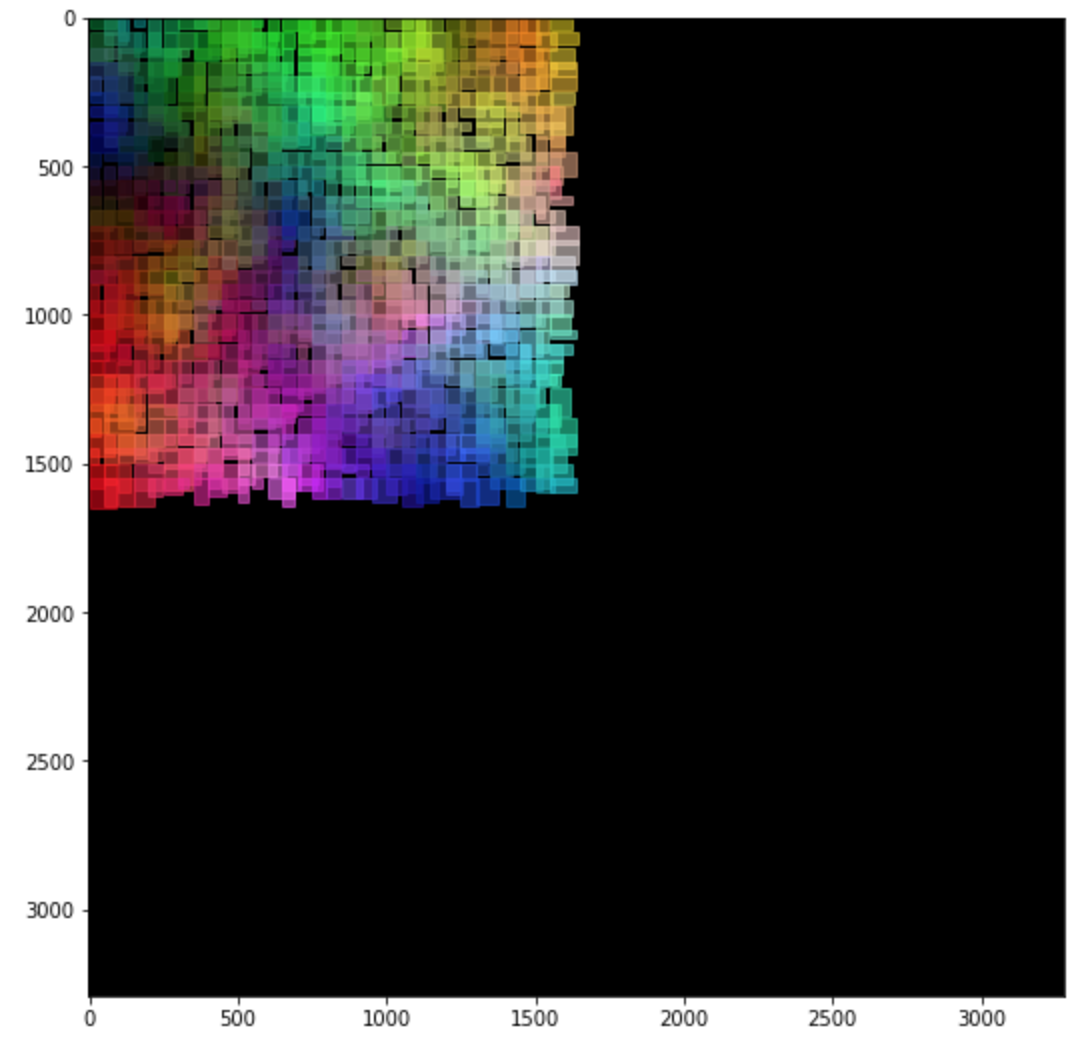
\includegraphics[height=0.6\textwidth]{./imgs/previous.png}}
    \caption{Die Positionen und der Rechtecke in ihrer ursprünglichen Anordnung. Die Rechtecke sind mit einer Transparenz von 0.6 Abgebildet, um die Überlagerungen mit den anderen Rechtecken sichtbar zu machen.}
    \label{fig:rwordle1}
\end{figure}
\begin{figure}[h]
    \noindent
  \makebox[\textwidth]{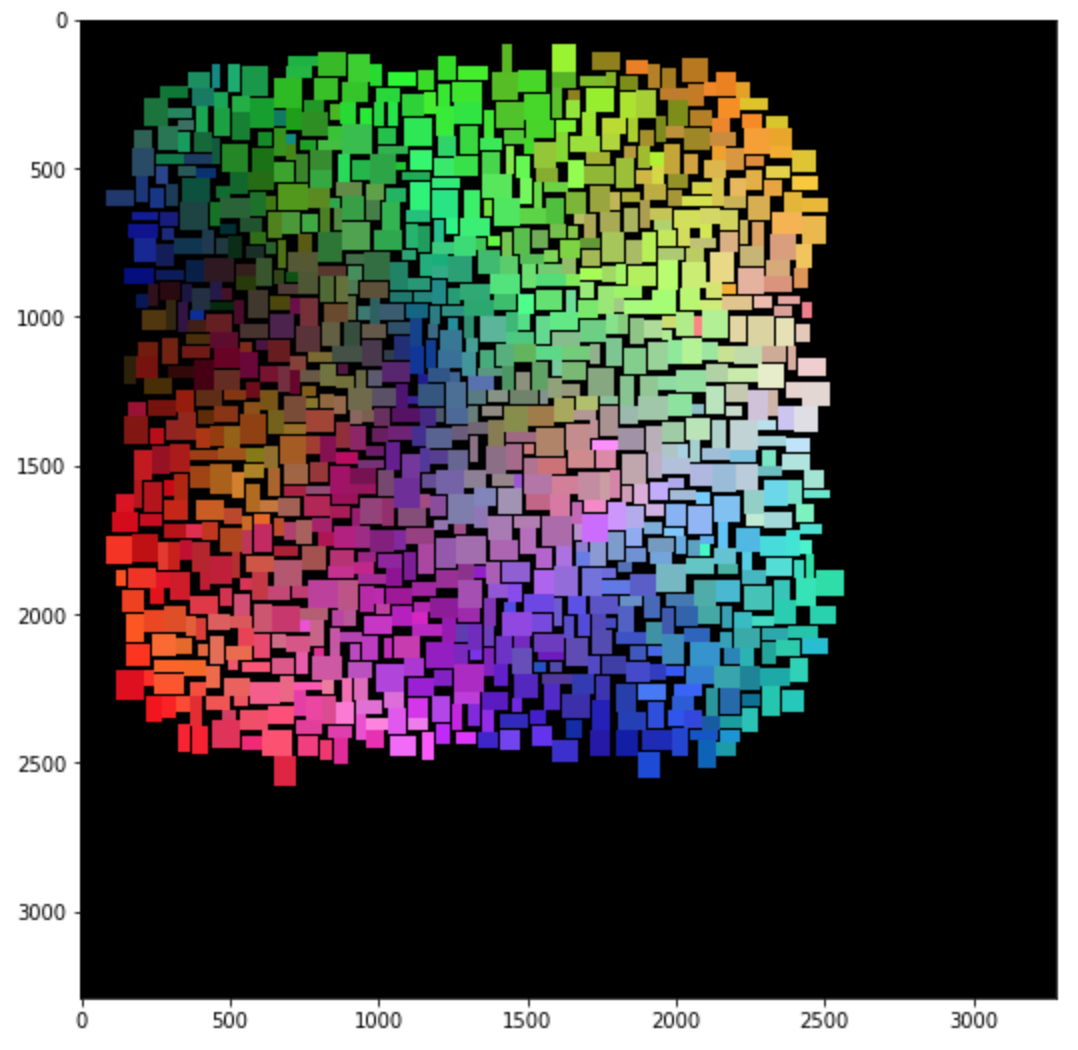
\includegraphics[height=0.6\textwidth]{./imgs/rwordle-concentric.png}}
    \caption{Die Anordnung der Rechtecke nachdem \textit{RWordle} mit einer konzentrischen Sortierung ausgeführt wurde}
    \label{fig:rwordle-kon}
\end{figure}
\begin{figure}[h]
    \noindent
  \makebox[\textwidth]{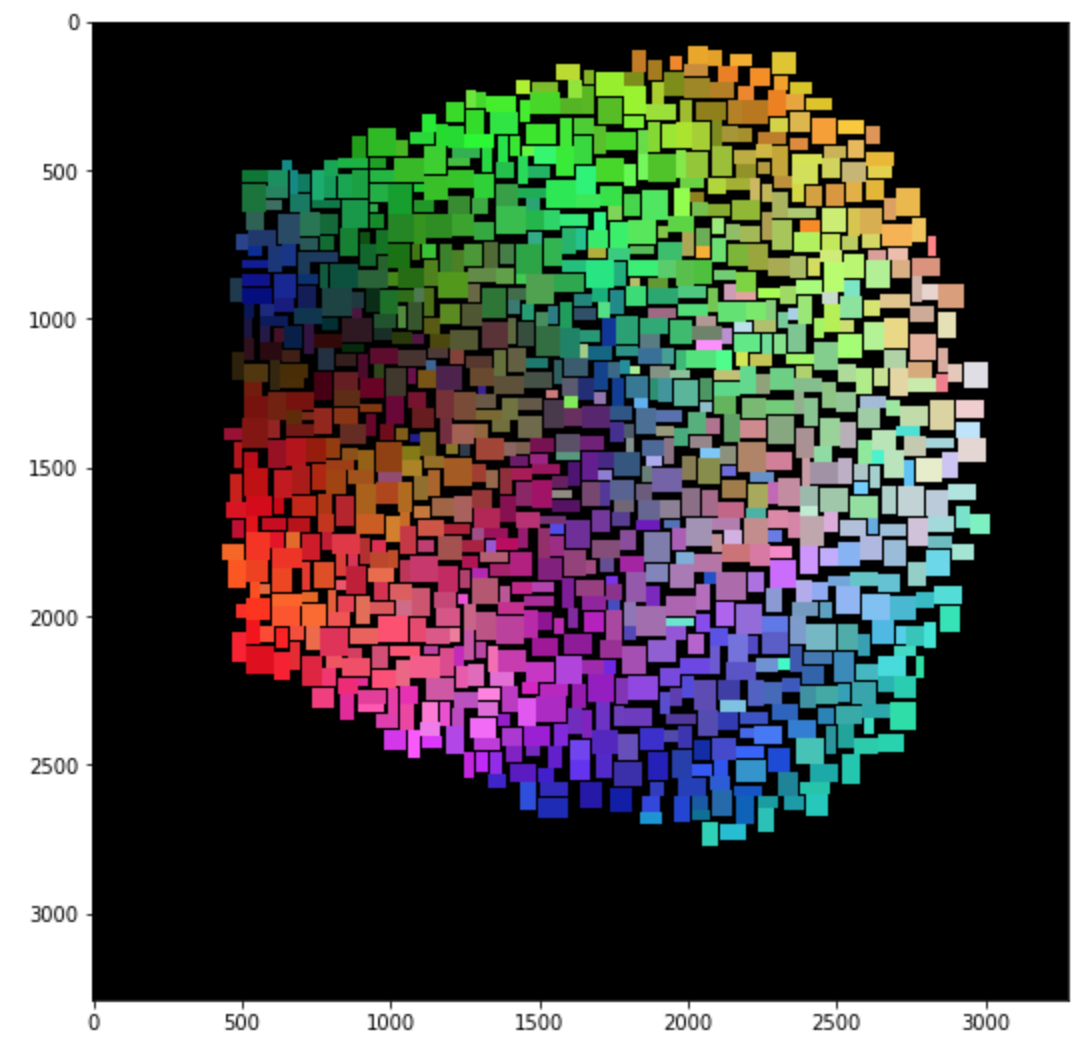
\includegraphics[height=0.6\textwidth]{./imgs/rwordle-linear.png}}
    \caption{Die Anordnung der Rechtecke nachdem \textit{RWordle} mit einer linearen Sortierung ausgeführt wurde}
    \label{fig:rwordle-lin}
\end{figure}
In der ersten Umsetzung wurde die SOM (siehe Abbildung \ref{fig:32som}), aus welcher ein Array mit Rechtecken zufälliger Größe erstellt wurde, verwendet. Die Rechtecke wurden außerdem leicht umpositioniert. Die implizite Position der Rechtecke kann als deren Position im Array verstanden werden. Da dies bei den Rechtecken dazu führt, dass eine sehr starke Überlappung auftritt, waren die ersten Ergebnisse von \emph{RWordle} nur mäßig gut. Die Ähnlichkeitsbeziehungen bleiben bei \emph{RWordle} relativ gut erhalten, jedoch kann die ursprüngliche Form, welche ein Quadrat ist, nicht gut erhalten werden. Es entsteht eine kreisförmige Anordnung der Rechtecke. Diese Anordnung ergibt sich nicht aus der konzentrischen oder linearen Vorsortierung, sondern aus der starken Überlagerung. Da die Rechtecke ausgehend von ihrer originalen Position einen neuen Platz ohne Überlagerung auf einem kreis- bzw. spiralförmigen Weg suchen, liegt der neue Platz immer möglichst nah an den bereits positionierten Rechtecken. Somit entsteht am Ende eine kreisförmige Anordnung, wenn die Rechtecke zuvor alle übereinander lagen und daher alle Rechtecke -- außer dem ersten Rechteck -- eine neue und insbesondere weit von ihrer ursprünglichen Position entfernten Position finden müssen. Hat man eine etwas aufgefächerte Anordnung der Rechtecke als Ausgangspunkt, kann die Form besser erhalten werden, da die ersten Rechtecke in der Anordnungsreihenfolge in ihrer neuen Position weniger von ihrer ursprünglichen Position abweichen. Dementsprechend weichen auch die Positionen der später bis zuletzt angeordneten Rechtecke weniger von ihrer ursprünglichen Position ab. Die Umpositionierung der Rechtecke von ihren zu stark überlappenden Position erfolgt über eine Skalierung der $x$- und $y$-Koordinate um einen gewissen Faktor. Wird dieser zu groß gewählt tritt keine Überlagerung mehr auf, aber der Platz zwischen den Rechtecken wird auch nicht minimiert. Daher ist eine so starke Überlagerung gesucht, bei deren Aufhebung durch \emph{RWordle} eine Anordnung entsteht, die der ursprünglichen Form noch ähnlich ist. 
%Da die Rechtecke durch die kreisförmige Suche um ihren Ausgangspunkt herum eine neue Position möglichst in der Nähe ihrer alten Position suchen, wird wenig von der ursprünglichen Anordnungsform abgewichen.
\begin{figure}[hp]
    \noindent
  \makebox[\textwidth]{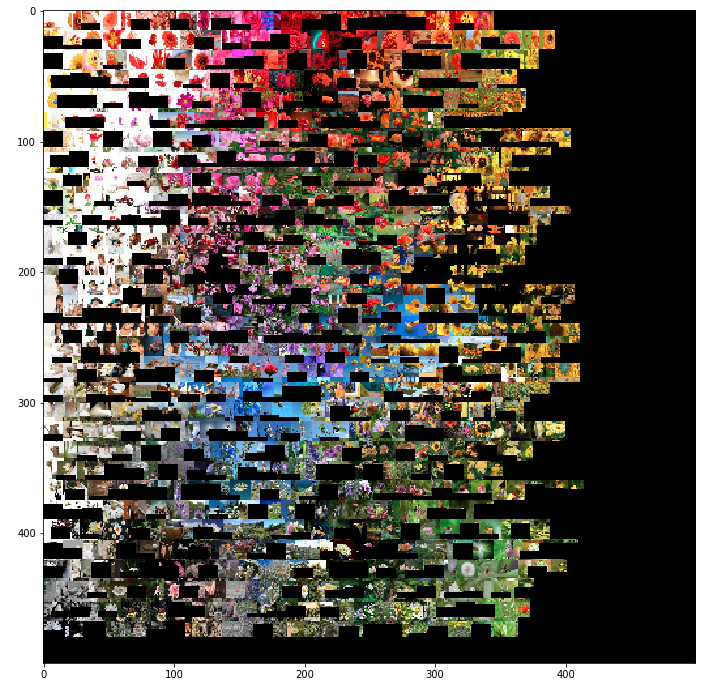
\includegraphics[width=0.75\textwidth]{./imgs/rwordle-flowers-simple.png}}
    \caption{Einfache Anordnung der Bilder nebeneinander.}
    \label{fig:rwordle-flower-simple}
\end{figure}
\begin{figure}[hp]
    \noindent
  \makebox[\textwidth]{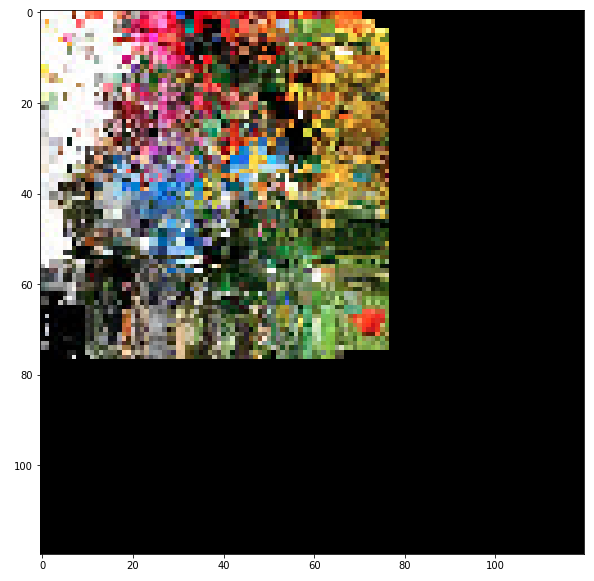
\includegraphics[width=0.75\textwidth]{./imgs/rwordle-flowers-overlap.png}}
    \caption{Starke Überlappung der Bilder vor der Anwendung von \textit{RWordle}.}
    \label{fig:rwordle-flower-overlap-strong}
\end{figure}
\begin{figure}[hp]
    \noindent
  \makebox[\textwidth]{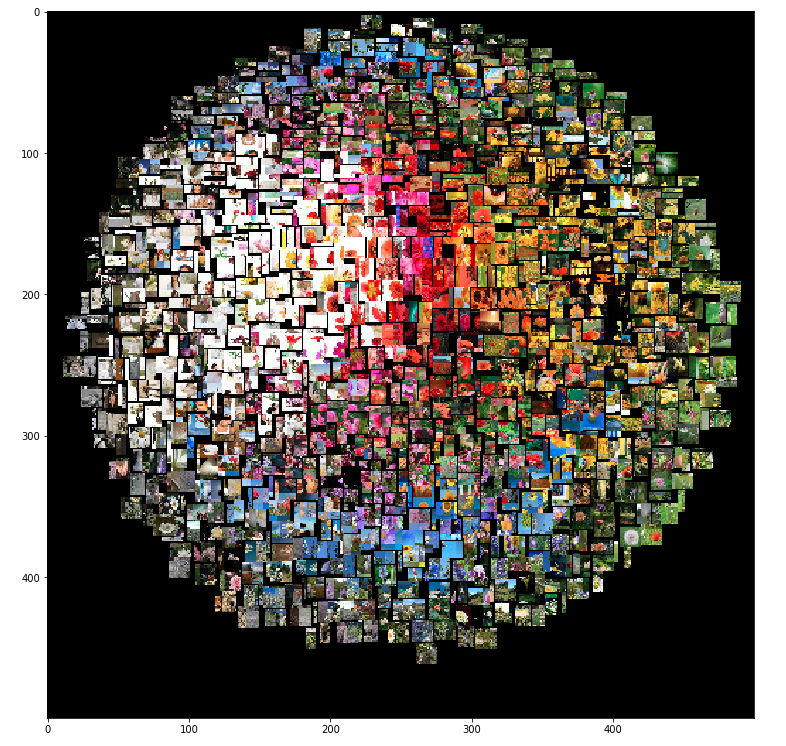
\includegraphics[width=0.75\textwidth]{./imgs/rwordle-flowers-concentric.png}}
    \caption{Anordnung der Bilder durch \textit{RWordle} mit einer konzentrischen Sortierung. Die Bilder haben sich zuvor stark überlappt und die Form der Bilderanordnung konnte nicht erhalten werden.}
    \label{fig:rwordle-flower-con1}
\end{figure}
\begin{figure}[hp]
    \noindent
  \makebox[\textwidth]{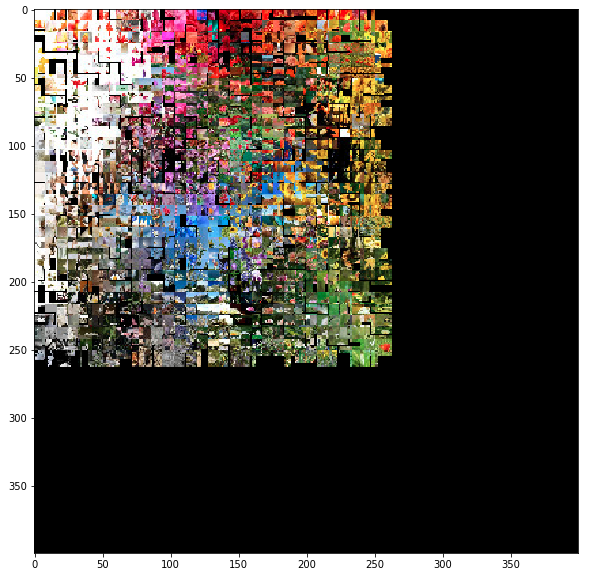
\includegraphics[width=0.75\textwidth]{./imgs/rwordle-flowers-overlap2.png}}
    \caption{Weniger starke Überlappung der Bilder vor der Anwendung von \textit{RWordle}.}
    \label{fig:rwordle-flower-overlap-less}
\end{figure}
\begin{figure}[hp]
    \noindent
  \makebox[\textwidth]{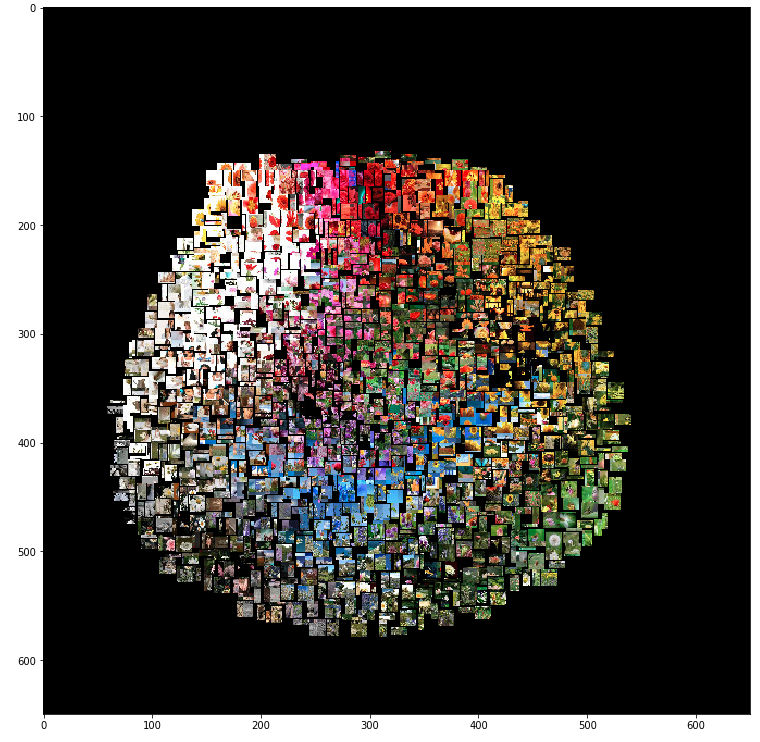
\includegraphics[width=0.75\textwidth]{./imgs/rwordle-flowers-concentric2.png}}
    \caption{Anordnung der Bilder durch \textit{RWordle} mit einer konzentrischen Sortierung. Die Bilder haben sich zuvor weniger stark überlappt (Abbildung \ref{fig:rwordle-flower-overlap-less}) und die Form der Bilderanordnung wurde etwas besser erhalten.}
    \label{fig:rwordle-flower-con2}
\end{figure}
\subsubsection{Erweiterung um Umsetzung mit Bildern}
Algorithmisch musste zur Anordnung mit Bildern nur wenig am Code verändert werden. Die Bilder mussten jedoch im Gegensatz zur Generierung der Rechtecke anders beschaffen werden. Dazu ist, wie in der Einleitung kurz erwähnt, ein Bild mit $32\times32$ sortierten Bildern gegeben. Diese sortierten Bilder sind in der gegebenen Form alle quadratisch. Für eine Eingabemenge, deren Bilder unterschiedliche Seitenverhältnisse haben, wird aus den quadratischen Bildern ein Teilbild ausgeschnitten. Für die Teilbilder wird ein Seitenverhältnis zwischen 1 bis 5 für die Höhe und 1 bis 5 für die Breite zufällig erzeugt. Diese Bilder sind zur Veranschaulichung einer nicht besonders gut geeigneten, jedoch einfach zu erzeugenden Anordnung, in Abbildung \ref{fig:rwordle-flower-simple} nebeneinander platziert worden.
%\pagebreak
\subsubsection{Die \texttt{updatePosition}-Funktion}
Um die Bilder oder Rechtecke neu zu positionieren wird die \texttt{updatePosition}-Funktion aufgerufen. Diese hat als Eingabeparameter das neu zu positionierende Rechteck bzw. Bild und einen Array, in dem die bereits positionierten Bilder enthalten sind. Um wie beschrieben eine neue Position kreis- bzw. spiralförmig um die ursprüngliche Position herum verlaufend zu finden, werden die Variablen \texttt{angle} bzw. \texttt{angle\_stepsize} und \texttt{radius} bzw. \texttt{radius\_stepsize} verwendet. Diese definieren, wie ihre Namen sagen, einen Winkel und einen Radius. Der Radius beschreibt letztlich den Abstand zur ursprünglichen Position. Diese Größen können beliebig klein oder groß skaliert werden. Es sollte darauf geachtet werden, dass der initiale Wert für \texttt{radius} und auch der Wert für \texttt{max\_radius} von der Größe, Anzahl und Verteilung der Bilder bzw. Rechtecke und die Größe der gegebenen Fläche abhängt und sinnvoll gesetzt werden müssen. \texttt{angle\_stepsize} und \texttt{radius\_stepsize} geben die Granularität vor, in der nach einer neuen Position gesucht wird. Je feiner diese ist, desto länger braucht man zur Positionierung der Bilder/Rechtecke.\\
%\begin{minipage}{\linewidth}
\begin{lstlisting}[language=Python, caption={\texttt{updatePosition}-Funktion zur Positionierung der Rechtecke für \emph{RWordle}},label=rot1]
def updatePosition(rect, layoutedRects):
    angle = 0
    angle_stepsize = pi/36
    radius = 5
    radius_stepsize = 5
    max_radius = radius_stepsize * 1000
    overlap = True
    
    while(overlap and radius <= max_radius): #iterate through each angle for radius increased by radius_stepsize until max_radius
        while(angle < 2*pi):
            tmpRect = ()
            tmpRect = tmpRect + ( (rect[0] + radius * cos(angle)), )
            tmpRect = tmpRect + ( (rect[1] + radius * sin(angle)), )
            for a in range(2, len(rect)):
                tmpRect = tmpRect + ( rect[a], )
            
            overlapping =  overlaps(tmpRect, layoutedRects[0])
            for i in range(1, len(layoutedRects)):
                #if any layouted rect still overlaps with new position of tmpRect
                overlapping = overlapping or overlaps(tmpRect, layoutedRects[i])
            
            if(not overlapping):
                overlap = False
                return tmpRect
            
            #otherwise update angle
            angle = angle + angle_stepsize
            
        #reset angle
        angle = 0
        radius = radius + radius_stepsize
\end{lstlisting}
%\end{minipage}

\subsubsection{Auswertung}
Im Vergleich zur Darstellung der Bilder/Rechtecke in aufgefächerter Form nebeneinander liefert \emph{RWordle} ein Ergebnis, welches in die gewünschte Richtung geht. Da \emph{RWordle} jedoch ein Algorithmus zur Entfernung von Überlagerungen in einer Menge von Objekten ist, hat er nur Auswirkungen auf Eingabemengen, in denen sich die Elemente tatsächlich überlagern. Er dient nicht in erster Linie der Anordnung von Bildern/Rechtecken in kompakter Form, es ist ein Resultat der Beseitigung der Überlagerung von Elementen und der Versuch die Anordnung und vorherige Position in Relationen zu den anderen Elementen so gut wie möglich beizubehalten. Wie in den Ergebnissen (siehe Abbildungen \ref{fig:rwordle-kon}, \ref{fig:rwordle-lin}, \ref{fig:rwordle-flower-con1}, \ref{fig:rwordle-flower-con2}) zu erkennen, werden die Nachbarschaften der Elemente insgesamt gut beibehalten.\\
Allerdings kann man vor allem bei kleineren Rechtecken/Bildern beobachten, dass diese die Nähe zu ihren urspünglichen Nachbarn nicht so gut aufrecht erhalten könne, da sie in Lücken hineinpassen, in die größere Rechtecke/Bilder nicht hineingepasst haben. Unter anderem bleibt ihre Position auf Grund von Umplatzierung der Elemente um sie herum unangetastet oder sie finden bei der Suche nach einer neuen Position freie Stellen, in die die ursprünglichen Nachbarn nicht hineingepasst haben und somit weiter entfernt ihre neue Position finden mussten.

\section{\textit{PicWall}}
In diesem Paper wird ein Algorithmus zur automatischen Erstellung von Fotokollagen auf unterschiedlich großen Flächen vorgestellt. Für ein gegebenes Seitenverhältnis einer rechteckigen Fläche soll eine solche Aufteilung gefunden werden, in der die gegebenen Bilder in ihren originalen Seitenverhältnissen angezeigt werden und dabei möglichst wenig Zwischenraum freilassen.

\subsection{Algorithmus}
Um eine passende Anordnung für eine Menge von Bilder mit unterschiedlichen Seitenverhältnissen in einer recheckigen Fläche zu finden, werden zwei grundlegende Funktionen benötigt. Zum einen die Berechnung von dem Seitenverhältnis der rechteckigen Fläche, welche sich aus den Seitenverhältnissen der Bilder ergibt, und zum anderen das Finden einer passenden Position in der Aufteilung der rechteckigen Fläche. 

Zur Umsetzung wird ein Divide-And-Conquer-Ansatz verfolgt, indem das Rechteck rekursiv randomisiert vertikal oder horizontal Aufgeteilt wird bis genügend Rechtecke entstehen, um alle gegebenen Bilder anzuzeigen. Diese Aufteilung wird in einer binären Baumstruktur widergespiegelt, wobei die Blätter die einzelnen Unterbereiche repäsentieren und die inneren Knoten die Information darüber beinhalten, ob eine vertikale oder horizontale Teilung der Fläche gegeben ist.

Nach der Unterteilung der gegebenen Fläche wird für jedes Blatt ein Bild gesucht, dessen Seitenverhältnis am besten zu dem Seitenverhältnis des Unterbereichs passt. In der Visualisierung wird das Bild so skaliert, dass es in den Unterbereich passt, jedoch ohne die Seitenverhältnisse zu verändern oder das Bild zu beschneiden.

Anfangs wird im Paper beschrieben, wie erst das rekursive Berechnen des gesamten Seitenverhältnisses erfolgt (siehe \emph{Algorithmus 1} in \cite{picwall}). Darauffolgend wird beschrieben, wie das Finden und Festlegen der am besten passenden Unterbereiche abläuft (siehe \emph{Algorithmus 2} in \cite{picwall}). Da dies noch keine optimale Lösung liefert und auch keine nutzerdefinierte Flächengröße sinnvoll aufgeteilt werden kann, wird dann auf Verbesserungen und Erweiterungen eingegangen. Zum einen lässt sich eine bessere Aufteilung ohne großen Aufwand finden, wenn für einen inneren Knoten mit zwei Blättern als Kinder die Bilder nicht einzeln pro Blatt bestimmt werden, sondern zwei Bilder gefunden werden, die gut in das Seitenverhältnis des inneren Knotens passen (siehe \emph{Algorithmus 3} in \cite{picwall}). Des Weiteren wird eine Aufbesserung der zufällig generierten horizontalen und vertikalen Aufteilung durch eine Iteration über den Baum, bei der jeder Knoten untersucht wird ob statt einer horizontalen oder vertikalen Aufteilung entsprechend eine vertikale oder horizontale Aufteilung besser zum erwarteten Seitenverhältnis passt. Sollte das der Fall sein, wird das Label im Knoten umgeschrieben und die Aufteilung der Fläche somit verbessert (siehe \emph{Algorithmus 4} in \cite{picwall}).

\subsection{Implementierung und Auswertung}


\begin{figure}[h]
\centering
\begin{minipage}{.45\textwidth}
  \centering
  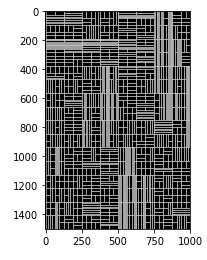
\includegraphics[width=0.9\textwidth]{./imgs/picwall-tree.png}
  \caption{Visualisierung der randomisierten Aufteilung in Unterbereiche}
  \label{fig:picwall-tree}
\end{minipage}%
\hfill
\begin{minipage}{.45\textwidth}
  \centering
  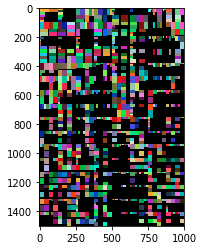
\includegraphics[width=0.9\textwidth]{./imgs/picwall-vis.png}
  \caption{Die Anordnung der Rechtecke/Bilder nachdem \textit{PicWall} ausgeführt wurde}
  \label{fig:picwall-vis}
\end{minipage}
\end{figure}

\section{Weitere untersuchte Algorithmen}\label{sec:weiter-algs}

\subsection{\emph{Tree-based Visualization and Optimization for Image Collection}}
In \emph{Tree-based Visualization and Optimization for Image Collection} \cite{treebased-vis} werden die Bilder gestreckt und gestaucht um eine möglichst lückenfreie Anordnung der Bilder zu erhalten. Die Ähnlichkeitsbeziehungen zwischen Bildern bleiben gut erhalten, da die Bilder einer zuvor erstellten Baumstruktur nach positioniert werden. Diese Baumstruktur zu erstellen wird beschrieben, aber es kann auch ein bereits erstellter Baum als Eingabe verwendet und visualisiert werden.

\subsection{\emph{Photo Layout with a Fast Evaluation Method and Genetic Algorithm}}
In \emph{Photo Layout with a Fast Evaluation Method and Genetic Algorithm} \cite{photo-layout} wird eine Methode vorgestellt, mit der man Collagen erstellen kann. Dabei wird das Seitenverhältnis beachtet und ebenfalls versucht die gegebenen Bilder möglichst lückenfrei anzuordnen. Ebenfalls wird erwähnt, dass es dem Nutzer möglich sein soll, ein besonderes Bild auszuwählen, welches größer als die anderen dargestellt werden soll. Die Andordnung der Bilder basiert auf einer binären Baumstruktur, die der von \textit{PicWall} sehr ähnlich ist. Allerdings wird ein geeigneter Baum basierend auf der \emph{Genetic Algorithm}-Methode gefunden, indem eine Menge unterschiedlicher binärer Bäume generiert wird und darunter dann der geeignetste ausgewählt wird. Eine Möglichkeit Ähn\-lich\-keits\-be\-zieh\-ung\-en zwischen den Bildern durch räumliche Nähe darzustellen wird nicht beschrieben.

\nocite{*}

\begin{thebibliography}{9}
  
\bibitem{nmap}
F. S. L. G. Duarte, F. Sikansi, F. M. Fatore, S. G. Fadel and F. V. Paulovich, 
\textit{Nmap: A Novel Neighborhood Preservation Space-filling Algorithm}, in IEEE Transactions on Visualization and Computer Graphics, vol. 20, no. 12, pp. 2063-2071, 31 Dec. 2014.
DOI: 10.1109/TVCG.2014.2346276,
URL: \url{http://ieeexplore.ieee.org/stamp/stamp.jsp?tp=&arnumber=6876012&isnumber=6935054}

\bibitem{nmapcode} Javascript Implementierung von Nmap \textit{nmap.js}, \url{https://github.com/sebastian-meier/nmap.js/}, 20.09.2018.

\bibitem{nmapclone} Geklonte und angepasste Implementierung von Nmap \textit{nmap.js}, \url{https://github.com/revialim/nmap.js}, 09.10.2018.

\bibitem{npm-get-pixels} NPM-Paket \texttt{get-pixels}, \url{https://www.npmjs.com/package/get-pixels}, 09.10.2018.

\bibitem{rwordle} H. Strobelt, M. Spicker, A. Stoffel, D. Keim, and O. Deussen. 2012. \textit{Rolled-out Wordles: A Heuristic Method for Overlap Removal of 2D Data Representatives.} Comput. Graph. Forum 31, 3pt3 (June 2012), 1135-1144. DOI=\url{http://dx.doi.org/10.1111/j.1467-8659.2012.03106.x}

\bibitem{picwall} Z. Wu and K. Aizawa, \textit{PicWall: Photo collage on-the-fly}, 2013 Asia-Pacific Signal and Information Processing Association Annual Summit and Conference, Kaohsiung, 2013, pp. 1-10.
DOI: 10.1109/APSIPA.2013.6694305,
URL: \url{http://ieeexplore.ieee.org/stamp/stamp.jsp?tp=&arnumber=6694305&isnumber=6694103}

\bibitem{treebased-vis} X. Han, C. Zhang, W. Lin, M. Xu, B. Sheng and T. Mei, \textit{Tree-Based Visualization and Optimization for Image Collection}, in IEEE Transactions on Cybernetics, vol. 46, no. 6, pp. 1286-1300, June 2016.
DOI: 10.1109/TCYB.2015.2448236,
URL: \url{http://ieeexplore.ieee.org/stamp/stamp.jsp?tp=&arnumber=7155544&isnumber=7466429}

\bibitem{photo-layout} J. Fan, \textit{Photo Layout with a Fast Evaluation Method and Genetic Algorithm}, 2012 IEEE International Conference on Multimedia and Expo Workshops, Melbourne, VIC, 2012, pp. 308-313.
DOI: 10.1109/ICMEW.2012.59,
URL: \url{http://ieeexplore.ieee.org/stamp/stamp.jsp?tp=&arnumber=6266273&isnumber=6266221}


\end{thebibliography}


\end{document}
